\subsection{Establish the project infrastructure: relevant standards/procedures, project team organization, roles/responsibilities, and communication methods.}

\subsubsection{Project Team Organization and Roles/Responsibilities}

\tasksubheading{Mô hình tổ chức nhóm dự án}

Nhóm dự án được tổ chức theo mô hình cấu trúc phẳng (\textit{Flat Structure}), phù hợp với quy mô 5 thành viên. Mô hình này hạn chế các tầng quản lý trung gian, cho phép các thành viên trao đổi trực tiếp, phối hợp giải quyết vấn đề và tham gia đóng góp vào các quyết định của dự án. Một thành viên đảm nhiệm vai trò quản lý dự án để điều phối công việc và theo dõi tiến độ; các thành viên còn lại chịu trách nhiệm về những lĩnh vực chuyên môn được phân công.

Những quyết định về kiến trúc và kế hoạch triển khai được thảo luận trong nhóm và ghi nhận trên Confluence. Những thay đổi ảnh hưởng đến phạm vi (\textit{scope}) hoặc \textit{Project Baseline} được nhóm đánh giá tác động và trình đại diện \textit{Client} xác nhận trước khi thực hiện.

Nhóm phân công mỗi thành viên phụ trách một vai trò chính, đồng thời hỗ trợ các công việc liên quan trong phạm vi chuyên môn phù hợp. Các lập trình viên kiêm nhiệm kiểm thử chéo và kiểm duyệt mã nguồn; BA hỗ trợ QA làm rõ các tình huống kiểm thử nghiệp vụ. Mỗi tác vụ trên Jira có một người chịu trách nhiệm chính và xác định người phối hợp hoặc kiểm tra khi cần thiết. Cách tổ chức này giúp phân định trách nhiệm rõ ràng mà vẫn duy trì tính linh hoạt trong quá trình thực hiện dự án.

Thành viên PM kiêm hỗ trợ Backend ở các phần việc cấu hình email, tạo dữ liệu giả lập, quản lý sự kiện, đăng ký/hủy, email, điểm danh thủ công và xuất CSV/Excel. Thành viên BA hỗ trợ thiết kế mockups, giao diện tài khoản/phân quyền và giao diện báo cáo. Mỗi tác vụ có một người thực hiện chính và người kiểm tra riêng; thời gian kiêm nhiệm được tính chung với công việc chính của cùng thành viên.

\tasksubheading{Cơ cấu tổ chức nhóm dự án}

Nhóm gồm 5 thành viên, tương ứng với 5 vai trò chính: Quản lý dự án (\textit{Project Manager -- PM}), Phân tích nghiệp vụ (\textit{Business Analyst -- BA}), Phát triển Backend, Phát triển Frontend và Đảm bảo chất lượng phần mềm (\textit{Quality Assurance -- QA/Tester}). PM và BA do hai thành viên riêng biệt đảm nhiệm. PM chịu trách nhiệm điều phối chung, trong khi các thành viên phối hợp trực tiếp với nhau để làm rõ yêu cầu, triển khai chức năng và kiểm tra chất lượng. Các vai trò được tổ chức theo cấu trúc phẳng, không hình thành nhiều tầng quản lý trung gian.

\begin{figure}[H]
\centering
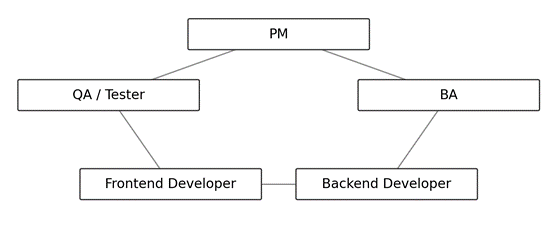
\includegraphics[width=0.82\textwidth]{Images/Picture1.png}
\caption{Cơ cấu phối hợp của nhóm dự án}
\label{fig:project-team-organization}
\end{figure}

Các đường nối trong Hình~\ref{fig:project-team-organization} minh họa quan hệ phối hợp giữa các vai trò, không thể hiện cấp bậc quản lý.

\tasksubheading{Vai trò và trách nhiệm}

\begin{itemize}
    \item \textbf{Quản lý dự án (Project Manager -- PM):} Chịu trách nhiệm lập kế hoạch, phân chia công việc và theo dõi tiến độ thực hiện trên Jira. PM phối hợp với các thành viên xác định mức độ ưu tiên của \textit{Backlog}, theo dõi những công việc bị chậm hoặc gặp trở ngại và điều chỉnh phân công phù hợp với năng lực của nhóm. Đồng thời, PM tổ chức hai buổi họp định kỳ mỗi tuần qua Google Meet, bảo đảm các vấn đề cần quyết định được đưa ra thảo luận và các kết luận quan trọng được cập nhật lên Confluence. Khi phát sinh yêu cầu mới, PM phối hợp với BA và đội ngũ kỹ thuật đánh giá tác động đến phạm vi, thời gian và nguồn lực trước khi thống nhất phương án xử lý. Bên cạnh công việc quản lý, PM tham gia thực hiện các phần việc Backend được phân công theo kế hoạch. Khi lập lịch, nhóm tính chung thời gian quản lý và thời gian lập trình của người PM để tránh phân công trùng thời điểm. Mã nguồn do PM tạo tuân thủ quy trình kiểm thử và Pull Request như các thành viên phát triển khác.

    \item \textbf{Phân tích nghiệp vụ (Business Analyst -- BA):} Chịu trách nhiệm tổng hợp, làm rõ và tài liệu hóa yêu cầu của hệ thống quản lý sự kiện. BA chuyển các yêu cầu đã thống nhất thành mô tả công việc hoặc \textit{User Story} có tiêu chí chấp nhận (\textit{Acceptance Criteria}) rõ ràng trên Jira, giúp lập trình viên và người kiểm thử hiểu thống nhất kết quả cần đạt. Các quy tắc nghiệp vụ như giới hạn số lượng đăng ký, thứ tự xử lý danh sách chờ, điều kiện chuyển sang danh sách chính thức và ghi nhận điểm danh được mô tả trên Confluence. BA cũng phối hợp với QA xây dựng các tình huống kiểm thử nghiệp vụ và đối chiếu sản phẩm với yêu cầu đã xác định. Ngoài phân tích nghiệp vụ và hỗ trợ kiểm thử, BA tham gia thiết kế mockups, lập trình giao diện tài khoản/phân quyền và giao diện báo cáo/tải tệp theo phân công. FE thống nhất cách kết nối API và review UI do BA thực hiện; QA kiểm thử các luồng hoàn chỉnh. BA vẫn giữ trách nhiệm làm rõ yêu cầu và tiêu chí chấp nhận.

    \item \textbf{Phát triển Backend (Backend Developer):} Chịu trách nhiệm đầu mối xây dựng phần xử lý phía máy chủ bằng Java Spring Boot, thiết kế cấu trúc dữ liệu và phát triển các API phục vụ ứng dụng. Backend Developer giữ đầu mối thống nhất thiết kế, API và tích hợp Backend; phụ trách tài khoản/phân quyền, giao dịch sức chứa/waitlist, xác thực QR và truy vấn báo cáo theo kế hoạch. BE thống nhất giao diện giữa các phần việc với PM và review Backend do PM thực hiện; PM nhận phần quản lý sự kiện, đăng ký/hủy, email, điểm danh thủ công và xuất tệp đã được xác định cụ thể. Backend Developer phối hợp với Frontend Developer để thống nhất cách trao đổi dữ liệu, cập nhật đặc tả API trên Confluence và xây dựng các kiểm thử đơn vị cho phần mã nguồn phụ trách. Mọi thay đổi được thực hiện trên nhánh riêng và gửi \textit{Pull Request} trên GitHub để thành viên khác kiểm duyệt trước khi sáp nhập.

    \item \textbf{Phát triển Frontend (Frontend Developer):} Chịu trách nhiệm đầu mối cấu trúc Angular, kết nối API và tích hợp giao diện; phụ trách các luồng sự kiện, đăng ký/waitlist và điểm danh. BA hỗ trợ các màn hình độc lập đã được phân công. FE thống nhất cách kết nối API và review mockups, mã UI do BA thực hiện cùng kết quả tích hợp trước khi chuyển kiểm thử. Thành viên phụ trách Frontend cũng thực hiện kiểm thử đơn vị phù hợp, cập nhật tiến độ trên Jira và tuân thủ quy trình \textit{Pull Request}, kiểm duyệt chéo trên GitHub.

    \item \textbf{Đảm bảo chất lượng và kiểm thử (Quality Assurance -- QA/Tester):} Chịu trách nhiệm lập các kịch bản kiểm thử dựa trên yêu cầu và tiêu chí chấp nhận đã thống nhất. Hoạt động kiểm thử tập trung vào tính đúng đắn của chức năng, sự phối hợp giữa giao diện và Backend, cũng như các luồng nghiệp vụ quan trọng như đăng ký, hủy đăng ký, tự động chuyển danh sách chờ và điểm danh bằng mã QR. QA ghi nhận lỗi trên Jira kèm các bước tái hiện, kết quả mong đợi và kết quả thực tế; sau khi lỗi được sửa, QA thực hiện kiểm thử lại và kiểm tra những chức năng liên quan. Vai trò này phối hợp với các thành viên đối chiếu điều kiện hoàn thành công việc theo \textit{Definition of Done} được quy định tại Mục~1.7.2.
\end{itemize}

\tasksubheading{Nguyên tắc kiêm nhiệm và kiểm tra chéo}

Nhóm thống nhất phân công 5 thành viên vào 5 vai trò chính như Bảng~\ref{tab:team-role-assignment}. Việc phân công một người phụ trách mỗi vai trò giúp xác định đầu mối chịu trách nhiệm rõ ràng; các nhiệm vụ hỗ trợ và kiểm tra chéo vẫn được thực hiện để duy trì khả năng phối hợp trong nhóm.

\begin{table}[H]
\centering
\renewcommand{\arraystretch}{1.2}
\begin{tabularx}{\textwidth}{|>{\centering\arraybackslash}p{2.2cm}|p{4.1cm}|X|}
\hline
\textbf{Thành viên} & \textbf{Vai trò chính} & \textbf{Nhiệm vụ phối hợp} \\
\hline
1 & PM & Kiêm hỗ trợ Backend theo tác vụ; vẫn điều phối, theo dõi và quản lý dự án \\
\hline
2 & BA & Hỗ trợ UI/Frontend: mockups, giao diện tài khoản/phân quyền, báo cáo; hỗ trợ kiểm thử nghiệp vụ \\
\hline
3 & Backend Developer & Đầu mối Backend; phối hợp và review phần PM thực hiện \\
\hline
4 & Frontend Developer & Đầu mối Frontend; phối hợp và review phần BA thực hiện \\
\hline
5 & QA/Tester & Phối hợp BA và Dev kiểm tra chất lượng \\
\hline
\end{tabularx}
\caption{Phân công vai trò chính và nhiệm vụ phối hợp}
\label{tab:team-role-assignment}
\end{table}

Bên cạnh trách nhiệm chính, các lập trình viên tham gia kiểm thử chéo và kiểm duyệt mã nguồn cho nhau trong phạm vi chuyên môn phù hợp. Người tạo \textit{Pull Request} không tự phê duyệt thay cho người kiểm duyệt độc lập; mã nguồn phải nhận được sự chấp thuận từ ít nhất một thành viên khác theo quy trình tại Mục~1.7.2. Việc lập trình viên tự kiểm thử phần việc của mình không thay thế hoạt động kiểm tra chéo hoặc kiểm thử tích hợp của nhóm.

Quy tắc kiểm duyệt độc lập áp dụng cả khi PM và BA kiêm lập trình: BE review Backend của PM; FE review mockups/UI của BA; QA review seed và kiểm thử độc lập. PM điều phối xử lý dựa trên kết quả kiểm tra. Người tạo không tự phê duyệt phần mình viết; vai trò quản lý hoặc phân tích nghiệp vụ không thay thế review kỹ thuật và kiểm thử.

Trách nhiệm ghi biên bản họp được luân phiên giữa các thành viên và xác định ở đầu mỗi buổi họp. Biên bản, quyết định và tài liệu nghiệp vụ được lưu trên Confluence; tiến độ và lỗi được theo dõi trên Jira; mã nguồn được quản lý trên GitHub. Zalo phục vụ trao đổi nhanh hằng ngày, còn Google Meet được sử dụng cho các buổi họp chính thức theo kế hoạch giao tiếp tại Mục~1.7.3.

\subsubsection{Relevant Standards and Procedures (Tiêu chuẩn và Quy trình dự án)}

Việc thiết lập các tiêu chuẩn và quy trình làm việc rõ ràng là nền tảng để bảo đảm tính nhất quán, minh bạch và chất lượng của sản phẩm phần mềm xuyên suốt vòng đời dự án. Nhóm áp dụng các quy trình quản lý và kỹ thuật sau:

\begin{itemize}
    \item \textbf{Quản lý dự án và tài liệu (Project and Documentation Management):} Dự án sử dụng hệ sinh thái Atlassian để quản lý tiến độ và tri thức. Jira Software được sử dụng làm công cụ cốt lõi để theo dõi vòng đời của từng tác vụ (\textit{Issue Tracking}), quản lý danh sách công việc (\textit{Backlog}) và phân công nguồn lực. Song song đó, Confluence, với phiên bản miễn phí hỗ trợ nhóm dưới 10 người, đóng vai trò là không gian lưu trữ tài liệu tập trung (\textit{Single Source of Truth}), nơi nhóm biên soạn và lưu trữ biên bản họp (\textit{Meeting Minutes}), đặc tả API và tài liệu kiến trúc hệ thống.

    \item \textbf{Quy trình quản lý mã nguồn (Version Control System):} Toàn bộ mã nguồn của dự án được lưu trữ và quản lý phiên bản tập trung trên GitHub. Nhóm áp dụng chiến lược phân nhánh \textit{Feature Branch Workflow} để bảo đảm tính ổn định của mã nguồn chính. Mọi tính năng mới hoặc bản vá lỗi phải được phát triển trên một nhánh riêng biệt (\textit{feature branch}) tách ra từ nhánh phát triển gốc. Mã nguồn chỉ được sáp nhập (\textit{merge}) thông qua \textit{Pull Request} sau khi hoàn thành các bước kiểm duyệt kỹ thuật.

    \item \textbf{Tiêu chuẩn công nghệ và lập trình (Coding Standards):} Dự án định hướng sử dụng Java Spring Boot cho hệ thống Backend nhằm hỗ trợ xử lý nghiệp vụ và bảo mật, kết hợp Angular cho nền tảng Frontend để xây dựng giao diện tương tác. Thành viên phải tuân thủ các quy chuẩn viết mã (\textit{Coding Conventions}) của từng ngôn ngữ, bao gồm quy tắc đặt tên biến/hàm, cấu trúc thư mục và các nguyên tắc \textit{Clean Code} nhằm nâng cao khả năng đọc hiểu và bảo trì mã nguồn.

    \item \textbf{Tiêu chuẩn nghiệm thu (Definition of Done -- DoD):} Một tác vụ lập trình chỉ được xem là hoàn thành (\textit{Done}) khi đáp ứng đầy đủ các điều kiện sau:
    \begin{itemize}
        \item mã nguồn biên dịch thành công và ứng dụng vận hành không phát sinh lỗi thực thi (\textit{runtime error}) trên môi trường phát triển;
        \item vượt qua các kịch bản kiểm thử đơn vị (\textit{Unit Test}) cơ bản;
        \item mã nguồn đã được đẩy (\textit{push}) lên GitHub và tạo \textit{Pull Request} hợp lệ;
        \item vượt qua quy trình kiểm duyệt chéo (\textit{Peer Code Review}) và nhận được sự chấp thuận (\textit{Approve}) từ ít nhất một thành viên khác trong nhóm.
    \end{itemize}
\end{itemize}

\begin{figure}[H]
\centering
\begin{tabularx}{\textwidth}{>{\centering\arraybackslash}X >{\centering\arraybackslash}X}
    
\includegraphics[height=2.4cm,keepaspectratio]{Images/Picture2.png} &
    
\includegraphics[height=2.4cm,keepaspectratio]{Images/Picture3.png} \\
    \textbf{Jira Software} & \textbf{Confluence}
\end{tabularx}
\vspace{0.3cm}
\caption{Các công cụ quản lý dự án và tài liệu được nhóm sử dụng}
\label{fig:project-management-tools}
\end{figure}

\subsubsection{Communication Methods (Phương thức giao tiếp)}

Để duy trì sự đồng bộ thông tin và bảo đảm khả năng phản ứng trước các rủi ro hoặc thay đổi yêu cầu, nhóm thiết lập kế hoạch giao tiếp (\textit{Communication Plan}) kết hợp giữa các kênh trao đổi tức thời và các buổi họp định kỳ.

\begin{itemize}
    \item \textbf{Kênh trao đổi hằng ngày (Daily Communication):} Nhóm sử dụng Zalo làm kênh giao tiếp nội bộ cho các hoạt động trao đổi tức thời. Kênh này được sử dụng để thông báo các cập nhật nhanh, trao đổi về các trở ngại kỹ thuật (\textit{blocker}) phát sinh trong quá trình phát triển và nhắc nhở tiến độ của các tác vụ trên Jira.

    \item \textbf{Kênh họp trực tuyến (Virtual Meetings):} Các cuộc họp chính thức nhằm báo cáo tiến độ, lập kế hoạch (\textit{Planning}) hoặc thảo luận giải pháp kỹ thuật được tổ chức qua Google Meet và sử dụng chức năng chia sẻ màn hình khi cần thiết.

    \item \textbf{Tần suất và nội dung cuộc họp (Meeting Cadence):} Nhóm duy trì hai buổi họp định kỳ mỗi tuần, mỗi buổi kéo dài trung bình 30 phút. Nội dung họp tập trung vào ba vấn đề: (1) báo cáo những công việc đã hoàn thành; (2) nhận diện và tháo gỡ các khó khăn hiện tại; và (3) thống nhất danh sách công việc của increment hiện tại hoặc tiếp theo. Các quyết định quan trọng được người ghi biên bản của buổi họp tổng hợp và cập nhật lên Confluence.

Sau khi Increment 1 hoàn thành kiểm thử, nhóm dự kiến sử dụng một buổi họp định kỳ để trình diễn bản thử nghiệm cho thầy Nguyễn Minh Tâm, với vai trò đại diện khách hàng, tại checkpoint CP1. PM thống nhất lịch demo, BA tổng hợp câu hỏi nghiệp vụ và cùng PM ghi nhận phản hồi vào Client Interaction Log. Nhóm gửi liên kết bản demo, phiên bản/build và các nội dung cần xác nhận qua Gmail; trao đổi trực tiếp có thể thực hiện qua Google Meet theo lịch đã thống nhất. Các phản hồi được đánh giá tác động trước khi điều chỉnh sản phẩm.
\end{itemize}

\begin{table}[H]
\centering
\renewcommand{\arraystretch}{1.2}
\begin{tabularx}{\textwidth}{|p{2.5cm}|p{3cm}|X|p{2.7cm}|}
\hline
\textbf{Kênh} & \textbf{Tần suất} & \textbf{Mục đích sử dụng} & \textbf{Nơi ghi nhận} \\
\hline
Zalo & Hằng ngày/khi cần & Cập nhật nhanh, trao đổi trở ngại và nhắc tiến độ & Jira hoặc Confluence nếu cần truy vết \\
\hline
Google Meet & 2 buổi/tuần, khoảng 30 phút/buổi & Báo cáo tiến độ, lập kế hoạch và thảo luận vấn đề cần quyết định & Biên bản trên Confluence \\
\hline
Gmail; Google Meet khi đã thống nhất lịch & Tại CP1 sau kiểm thử I1 và khi cần xác nhận yêu cầu/thay đổi & Gửi bản demo và câu hỏi cần xác nhận; tiếp nhận phản hồi, làm rõ tác động và quyết định & Client Interaction Log trên Confluence; liên kết email/biên bản tương ứng \\
\hline
Jira & Cập nhật theo tác vụ & Quản lý \textit{Backlog}, phân công, tiến độ và lỗi & Jira \\
\hline
Confluence & Cập nhật sau họp hoặc khi tài liệu thay đổi & Lưu biên bản, quyết định, yêu cầu, đặc tả API và kiến trúc & Confluence \\
\hline
GitHub & Theo hoạt động phát triển & Quản lý mã nguồn, \textit{Pull Request} và kiểm duyệt chéo & GitHub \\
\hline
\end{tabularx}
\caption{Kế hoạch giao tiếp của nhóm dự án}
\label{tab:communication-plan}
\end{table}